% ==============================================================================
% examples/titlepage_template.tex — หน้าปกในเวกเตอร์สไตล์ Dark Mode (TikZ 100%)
% แม่แบบมาตรฐานจากทักษะ academic-book-cover-architect
% ==============================================================================
\begin{titlepage}
\thispagestyle{empty}
\centering
\begingroup
\pagecolor{black!94}
\color{white}

\vspace*{0.24in}

{\fontsize{9}{12}\selectfont\bfseries\color{green!45!yellow}
[FIELD BADGE / สาขาวิชาการ] \enspace / \enspace [SPECIALIZATION]}

\vspace{0.12in}
{\color{green!45!yellow}\rule{0.78in}{1.2pt}}

\vspace{0.16in}
{\fontsize{13}{17}\selectfont\bfseries
[ชื่อเรื่องภาษาไทย บรรทัดที่ 1]}

\vspace{0.03in}
{\fontsize{22}{27}\selectfont\bfseries
[ชื่อเรื่องภาษาไทย บรรทัดที่ 2]}

\vspace{0.07in}
{\fontsize{10}{13}\selectfont\color{white!75}
([English Textbook / Manual Title])}

\vspace{0.13in}

% ภาพประกอบเวกเตอร์แท้ 100% วาดด้วย TikZ Bezier Curves
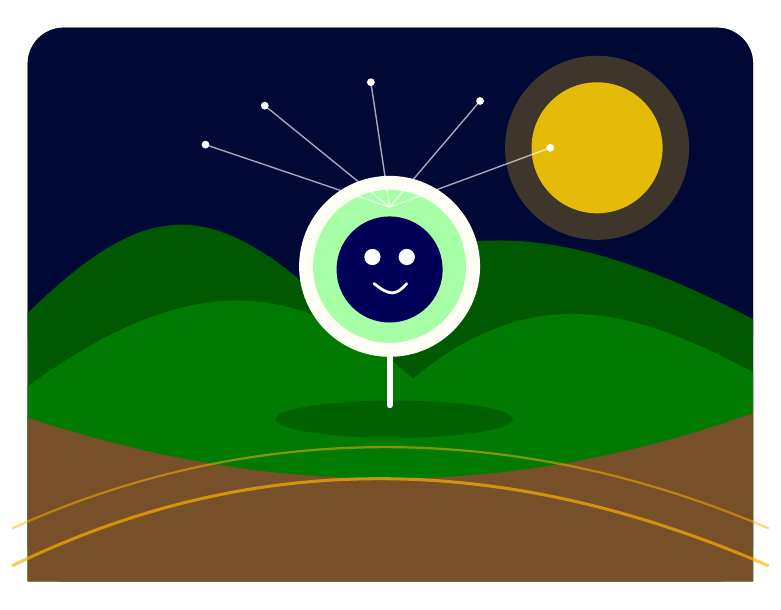
\begin{tikzpicture}[x=0.78in,y=0.78in]
  \useasboundingbox (0,0) rectangle (4.65,3.55);

  % ท้องฟ้ายามค่ำ/สนธยา
  \fill[rounded corners=13pt,green!12!black]
    (0,0) rectangle (4.65,3.55);
  \fill[rounded corners=13pt,blue!30!black,opacity=.72]
    (0,1.35) rectangle (4.65,3.55);
  \fill[yellow!70!orange,opacity=.88] (3.65,2.78) circle (.42);
  \fill[yellow!55!orange,opacity=.25] (3.65,2.78) circle (.59);

  % ทิวเขาระยะไกลและระยะใกล้
  \fill[green!35!black]
    (0,1.72) .. controls (.75,2.45) and (1.16,2.48) .. (1.92,1.78)
    .. controls (2.64,2.37) and (3.48,2.3) .. (4.65,1.68)
    -- (4.65,0) -- (0,0) -- cycle;
  \fill[green!48!black]
    (0,1.25) .. controls (1.03,2.00) and (1.73,1.95) .. (2.47,1.30)
    .. controls (3.23,1.93) and (3.87,1.76) .. (4.65,1.34)
    -- (4.65,0) -- (0,0) -- cycle;

  % แปลงปลูกโค้งและแปลงดิน
  \fill[brown!62!black]
    (0,0) -- (4.65,0) -- (4.65,1.08)
    .. controls (3.12,.53) and (1.6,.52) .. (0,1.05) -- cycle;
  \draw[orange!60!yellow,opacity=.68,line width=1.1pt]
    (-.1,.10) .. controls (1.40,.83) and (3.00,.86) .. (4.75,.10);
  \draw[orange!60!yellow,opacity=.52,line width=.8pt]
    (-.1,.34) .. controls (1.42,1.03) and (3.12,1.04) .. (4.75,.34);

  % อุปกรณ์เซนเซอร์อัจฉริยะ / วัตถุเด่นตรงกลาง
  \fill[black,opacity=.2] (2.35,1.04) ellipse (.76 and .12);
  \draw[white!70,line width=2.2pt,line cap=round] (2.32,1.13) -- (2.32,1.55);
  \fill[white!96!yellow] (2.32,2.02) circle (.58);
  \fill[green!35!white] (2.32,2.02) circle (.49);
  \fill[blue!35!black] (2.32,2.00) circle (.34);
  \fill[white] (2.21,2.08) circle (.052);
  \fill[white] (2.43,2.08) circle (.052);
  \draw[white,line width=1pt,line cap=round]
    (2.22,1.91) .. controls (2.32,1.83) and (2.36,1.83) .. (2.43,1.91);

  % ต้นกล้าและเครือข่ายสัญญาณ IoT
  \foreach \x/\y in {1.14/2.80,1.52/3.05,2.20/3.20,2.90/3.08,3.35/2.78} {
    \draw[white!60,opacity=.65,line width=.5pt] (\x,\y) -- (2.32,2.40);
    \fill[white!90] (\x,\y) circle (.025);
  }
\end{tikzpicture}

\vspace{0.08in}

{\fontsize{9}{12}\selectfont\bfseries\color{green!45!yellow}
[เอกสารประกอบการสอน / ตำราเรียน / สื่อการเรียนรู้ดิจิทัล]}

\vfill

{\color{green!45!yellow}\rule{0.72in}{1pt}}\\[0.10in]
{\fontsize{15}{19}\selectfont\bfseries ผู้ช่วยศาสตราจารย์ ดร.ชีวะ ทัศนา}\\[0.04in]
{\fontsize{10}{13}\selectfont\color{white!75}
สาขาวิชาปัญญาประดิษฐ์เพื่อเกษตรดิจิทัลและสิ่งแวดล้อม}\\
{\fontsize{10}{13}\selectfont\color{white!75}
คณะวิทยาศาสตร์และเทคโนโลยี}\\
{\fontsize{10}{13}\selectfont\color{white!75}
มหาวิทยาลัยราชภัฏรำไพพรรณี}

\vspace{0.14in}
{\fontsize{9}{12}\selectfont\color{white!60}
โครงการพัฒนาการเรียนการสอนและวิจัยนวัตกรรม}\\
{\fontsize{10}{13}\selectfont\bfseries\color{green!45!yellow}พ.ศ. 2569}

\vspace*{0.16in}
\endgroup
\end{titlepage}
\pagecolor{white}
\cleardoublepage
